A parallel version of AFGMiner benefits from the multiple cores available in many computing systems. An important challenge in the implementation of a parallel version of AFGMiner-locreg, {\bf p-AFGMiner}, is the distribution of the workload to improve load balancing.
\REM{
AFGMiner-locreg executes the following steps while a queue $Q$ of heavyweight patterns to be extended is not empty: (i) collect all distinct heavyweight attributes that belong to the $k$-edge patterns in $Q$, and insert them into $A_{k + 1}$; (ii) extend the patterns and test their children to generate a set of heavyweight child patterns $C$ that have one additional edge in comparison to patterns already in $Q$; (iii) add elements from $C$ into the output set to be returned to the user; and (iv) add elements from $C$ into $Q$. Patterns of $(k + 1)$ edges, one by one, become head-of-queue, and thus go through the steps described above, when all patterns of $k$ edges have been similarly processed and removed from the queue. A pattern $p$ is \emph{dependent} on a pattern $q$ if $p$ is extended from $q$. Therefore, $q$ needs to be mined and its support value determined before $p$ is processed. The set of patterns that have the same number of edges forms a \emph{generation}. There are no dependencies among patterns of the same generation. That is because each $k$-edge pattern depends only on its parent pattern and on $A_k$, which contains the distinct attributes from the previous generation, or, if $k = 0$, the possible attributes from $A$. Therefore, the processing of patterns belonging to the same generation can be safely divided amongst different threads. 
}
p-AFGMiner executes the following steps while a queue $Q$ of heavyweight patterns is not empty (s signals a sequential step, while p signals a parallel step): (i-s) fork into $n$ threads to start the processing of a new generation composed of patterns with $k$ edges.

For $k = 0$, (ii-s) divide the set $A_0$ among the threads and (iii-p) each thread generates 0-edge candidate patterns using their part of $A_0$ and searches the database for these patterns --- heavyweight patterns form a local queue $Q_{TL}$ and the set of attributes in $Q_{TL}$ form $A_{TL}$, the local set of attributes.

For $k > 0$, (ii-s) distribute the queue $Q$ of $k$-edge heavyweight patterns among $n$ thread-local queues $Q_{TL}$; (iii-p) each thread generates $(k+1)$-edge candidates from patterns in $Q_{TL}$ and computes their support, generating $A_{TL}$ and adding the patterns found to be heavyweight to $Q_{TL}$; 

Then: (iv-s) synchronize when all threads finish step (iii) and unify all $Q_{TL}$s into a single queue $Q$, and all $A_{TL}$s into a single $A_{k+1}$ set of attributes; and (v) start processing the next generation, if $Q$ is not empty. The dataset of AFGs, $DS$, is read-only during the entire run of p-AFGMiner, allowing the maintenance of thread-local versions of variables and thus reducing synchronization.

The distribution of $Q$ among threads should balance the workload to improve the performance of p-AFGMiner. The number of occurrences of the parent of a pattern $p$ in $DS$ is the most important factor determining the time required to search for occurrences of $p$. A reasonable heuristic tries to balance the number of parent-pattern occurrences assigned to each thread. 

\begin{figure}[h!]
\centering
    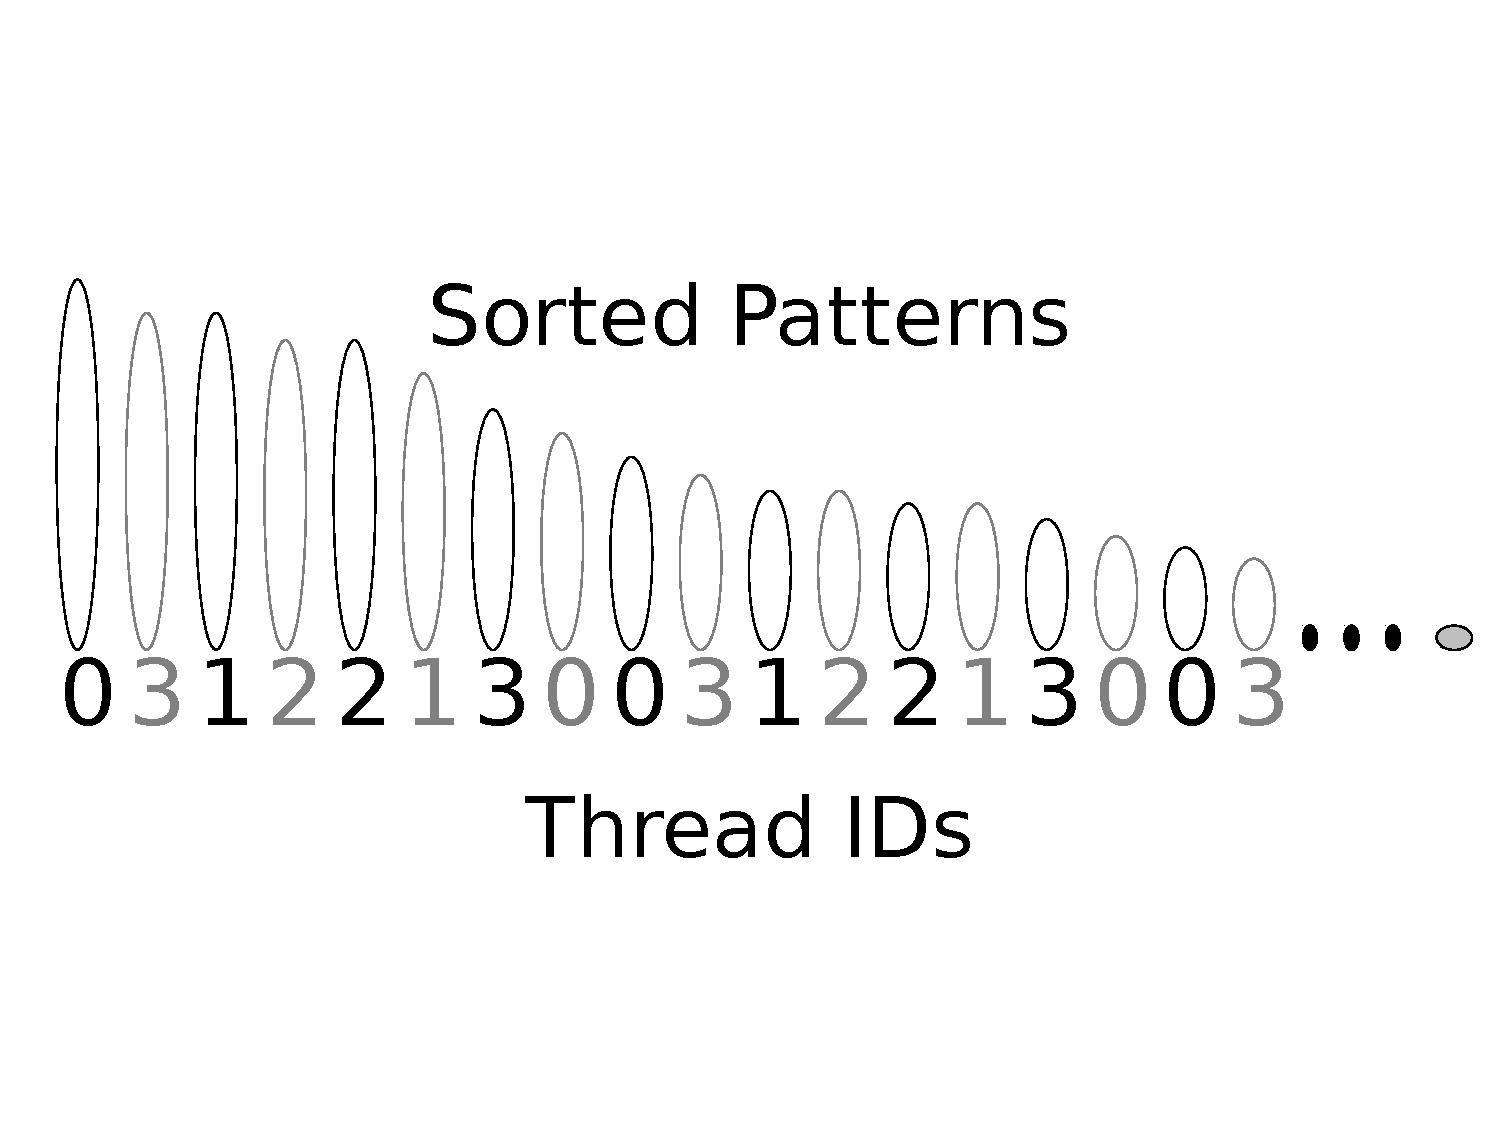
\includegraphics[scale=0.2]{figures/WorkDistributionHeuristic.pdf}
    \caption{Illustration of pattern distribution heuristic.}
    \label{fig:WorkDistributionHeuristic}  
\end{figure}

The pattern-distribution heuristic created for p-AFGMiner sorts the $m$ patterns in $Q$ by decreasing order of the number of parent-pattern occurrences. The heuristic then does a round-robin assignment of patterns to threads following an increasing order for the patterns with an even position in the sorted $Q$ and in decreasing order for patterns with an odd position in the sorted $Q$ as illustrated in Figure~\ref{fig:WorkDistributionHeuristic} --- assume that numbering in $Q$ starts at zero. In this illustration each ellipse represents a pattern in $Q$ and the size of the ellipse stands for the number of occurrences of the pattern's parent in the database.
This simple $O(n)$ heuristic is effective for a moderate number of threads and for limited variations in the number of parent-pattern occurrences. Experimental evaluation revealed that this workload-distribution heuristic lowered the execution time of p-AFGMiner, on average, by 6\% when compared with a naive workload distribution method that simply distributes patterns among the threads without any sorting.


 


 
